% ---------------------------------------------------------------------------
% Centri — IEEE conference draft (first pass).
%
% Per direction (2026-08-03):
%   * ABSTRACT is skipped (placeholder below).
%   * RELATED WORK is a CONDENSED version: the two works Centri is positioned
%     against directly (Utami dissertation, P-MAGIC) are written; the wider
%     video / question-generation line is still a stub.
%   * Everything else is a real draft on real numbers from the 7-clip sweep.
%
% All numbers are traceable; see \todo notes for the few that need a decision.
% Compile: pdflatex -interaction=nonstopmode centri-ieee.tex (twice)
% ---------------------------------------------------------------------------
\documentclass[conference]{IEEEtran}
\IEEEoverridecommandlockouts

\usepackage{cite}
\usepackage{amsmath,amssymb}
\usepackage{graphicx}
\usepackage{booktabs}
\usepackage{multirow}
\usepackage{xcolor}
\usepackage{url}
\usepackage[hidelinks]{hyperref}
\usepackage{algorithm}
\usepackage[noend]{algpseudocode}
\usepackage{tikz}
\usetikzlibrary{arrows.meta,positioning,fit,backgrounds}

\graphicspath{{../presentation/figs/}{../technical-report/figures/}}

\newcommand{\todo}[1]{{\color{red}\textbf{[TODO: #1]}}}
\newcommand{\ac}{a_{c}}
\newcommand{\at}{a_{t}}

\begin{document}

% Title from the 2026-07-08 meeting note (note-7-8), candidate #3, tightened:
% dropped "An investigation of" and the trailing "support" to fit two lines.
\title{LLM-Based Generation and Evaluation of Authentic\\
Physics Learning Material from Video Recognition\\
with Multimodal Annotation}

\author{\IEEEauthorblockN{\todo{authors}}
\IEEEauthorblockA{\todo{Department, National Central University, Taiwan}\\
\todo{email}}}

\maketitle

% ---------------------------------------------------------------------------
% ---------------------------------------------------------------------------
% ABSTRACT — intentionally empty per direction (2026-08-03). Write last.
% Working one-liner kept here so it is not lost:
%   Centri turns a phone video of a spinning everyday object into measured
%   kinematics and three difficulty-tiered, figure-annotated physics
%   worksheets, with a deterministic grounding gate and a four-layer
%   evaluation; on a seven-clip corpus the tier ladder reproduces across two
%   independent LLM raters while no absolute judge score does.
% ---------------------------------------------------------------------------
\begin{abstract}
\end{abstract}

\begin{IEEEkeywords}
automatic content generation, physics education, video analysis, difficulty
tiering, LLM-as-a-judge, multimodal evaluation
\end{IEEEkeywords}

% ===========================================================================
\section{Introduction}
% ===========================================================================
% INTRODUCTION — intentionally empty per direction (2026-08-03).
% The drafted version is preserved below, commented out. It argued three
% claims: (1) video suffices as the measurement front end; (2) difficulty can
% be tiered deterministically and the ladder measured; (3) evaluation layers
% see different failures and no single layer is sufficient. Uncomment and
% edit, or rewrite from Sec. V.
%
%
%
% Authentic learning material---material built from an object the learner has
% actually seen move---is expensive to produce because somebody has to measure
% the object. Systems that automate this have so far attached a sensor to the
% thing being measured, or asked the learner to mark the motion frame by frame.
% Both work, and both narrow the set of situations in which a teacher can
% generate material at all: a phone taped to a ceiling fan is not a lesson plan.
%
% \textbf{Centri} takes the other route. A learner points a phone at something
% turning---a ceiling fan, a record turntable, a playground roundabout---and
% uploads the clip. Nothing is attached to the object and nothing is marked by
% hand. The system localises and tracks the moving object, fits its orbit,
% recovers the angular kinematics, and writes three parallel physics worksheets
% at increasing cognitive demand, each with figures drawn onto the footage
% itself. Every number in every worksheet is verified against the measurement
% before the document is rendered.
%
% The engineering claim is narrow and the evaluation claim is narrower. This
% paper argues three things.
%
% \begin{enumerate}
% \item \textbf{Video suffices as the measurement front end for generated
% physics material.} On the one clip for which we hold an independent sensor
% log, time-averaged quantities agree with a phone gyroscope to within
% $0.1$--$0.5\%$, while per-instant angular velocity carries about $4\%$ RMS
% error. That split---averages trustworthy, instants not---determines what the
% generated material is allowed to say, and the system enforces it rather than
% hoping for it.
%
% \item \textbf{Difficulty can be tiered deterministically and the ladder can be
% measured.} Tiers are defined by which fields of the measurement seed a passage
% may draw on, not by asking a model to ``write it harder.'' Element
% interactivity, a cognitive-load measure computed from the finished prose,
% rises strictly across the three tiers on $7$ of $7$ clips. Flesch--Kincaid
% reading grade rises on $1$ of $7$, and we report that rather than suppress it:
% the level whose difficulty is carried by symbols reads as the easiest prose.
%
% \item \textbf{Evaluation layers see different failures, and no single layer is
% sufficient.} We report a deterministic grounding gate, reference-based
% similarity metrics, two independent LLM judges on a 12-criterion rubric, and a
% vision-capable judge on an 11-criterion multimodal rubric. Each layer in this
% study caught at least one defect that every other layer passed---including a
% tracker artifact that inflated one clip's published centripetal acceleration
% by $27\%$, and a figure caption asserting an object was at rest while its own
% plotted curve showed $24$~rad/s. We also report the reliability of the judge
% layer itself: two raters on a byte-identical prompt reach
% $\kappa = 0.34$ quadratic-weighted, agree on the tier ordering, and agree on
% nothing at all about grounding accuracy ($\kappa = -0.04$).
% \end{enumerate}
%
% The third point is the one we would most like to be read. Automatic evaluation
% of generated educational material is converging on LLM judges, and a single
% judge run produces a number that looks like a measurement. On our corpus it is
% not one.
%
% ===========================================================================
\section{Related Work}
\label{sec:related}
% ===========================================================================
\todo{Condensed. A fuller treatment of the video / question-generation line is
deferred; the two works Centri must be positioned against directly are
covered here.}

\subsection{The parent line: authentic problem generation}

Centri descends from a line of work on generating \emph{authentic} problems
from real-world context. Utami's dissertation~\cite{utami} is its immediate
parent: a systematic review of 28 automatic word-problem generation studies
(2015--2025), followed by Geo-QG, which acquires context through mobile object
recognition and AR-Core measurement and generates geometry problems at three
difficulty levels, and by a group-socialization generator.

Three findings of that review define the gap Centri occupies. The field is
dominated by arithmetic ($50\%$) and algebra ($25\%$), with geometry at $11\%$
and physics essentially absent. \emph{Every} reviewed study takes text as
input; a handful add images, and none measure kinematics from video. And only
$3$ of $28$ generate with explicit difficulty levels at all.

One difference must be stated plainly so that a reader from this line is not
misled. Utami's difficulty semantics are \emph{structural}---easy is one
object, intermediate compares two, advanced treats a compound shape---whereas
Centri's are \emph{depth-based}: one idea, then several coordinated relations,
then integration over time. Both are legitimate difficulty ladders; they are
not the same axis, and results are not directly comparable across them.
P-MAGIC's tiers sit closer to Utami's than to ours on this point---its advanced
level is defined as \emph{comparing two scenarios}---even though all three
systems map their tiers onto the same revised Bloom taxonomy~\cite{bloom} and
the same Indonesian upper-secondary curriculum.

\subsection{The sibling system: sensing through a phone IMU}

P-MAGIC~\cite{pmagic} is the closest system to Centri and shares its advisor
and its evaluation instrument. It generates multimodal physics word problems
about circular motion, annotates a still frame with radius and acceleration
vectors, labels increase/steady/decrease phases on graphs and tables, and was
evaluated by ten senior high-school physics teachers on a modality-organised
rubric of $22$ criteria, scored $1$--$10$ and reported over $25$ rows (the $22$
plus three combined-modality relevancy scores), reaching relevancy means of
$8.58$, $8.21$ and $8.18$ at their three levels. Their automatic layer is
BERTScore, semantic textual similarity, and an LSTM fluency model, correlated
against the teacher scores by Pearson $r$; generation and object recognition
both run on a commercial cloud model.

Because P-MAGIC is already multimodal and already annotated, \textbf{neither
multimodality nor annotation is Centri's novelty against the parent line}, and
we do not claim them as such. Four differences are real:

\begin{itemize}
\item \textbf{Sensing.} P-MAGIC reads a phone's accelerometer and gyroscope
with the phone attached to the moving object. Centri measures the real
object's motion from ordinary video with nothing attached, which is both more
ubiquitous and applicable to objects one cannot bolt a phone to---a ceiling
fan, a playground roundabout.
\item \textbf{Unit of output.} P-MAGIC generates word \emph{problems}; Centri
generates tiered expository \emph{material} with embedded interaction. This is
why several rows of the shared rubric that presuppose a solvable task are
dropped here rather than scored.
\item \textbf{Grounding.} Centri verifies every number, relation, phase label
and figure annotation against the measurement before rendering
(Sec.~\ref{sec:gate}); the parent line has no deterministic equivalent.
\item \textbf{Annotation across the motion} rather than on one still image
plus a sensor graph. P-MAGIC annotates by Hough transform and classical CV on
the image, and labels graph and table phases by thresholding a moving-window
standard deviation and slope. Its own ablation---six conditions, $N = 40$
each---reports every annotated modality beating its unannotated counterpart
(image $0.895$ vs $0.839$, table $0.871$ vs $0.822$, graph $0.859$ vs $0.825$;
Cohen's $d$ up to $1.7$). Two cautions on reading those numbers, since we rely
on them: they are \emph{automatic} semantic-relevancy scores on a $0$--$1$
scale, not teacher ratings and not learning outcomes; and the accompanying
claim that image-bearing modalities outperform graph- and table-only ones rests
on $2$ of $15$ pairwise comparisons reaching $p < .05$. Read narrowly, it is
still the best available motivation for doing annotation well---which is what
we take from it, rather than a claim of novelty.
\end{itemize}

We adopt P-MAGIC's rubric and reporting layout deliberately, so that the two
systems' results tables can be read side by side, and we mark as \texttt{n/a}
the one automatic metric we cannot reproduce because its trained weights are
not published.

\subsection{Video in physics education}

Video analysis is established physics pedagogy, but it is \emph{manual}: tools
in the Tracker / Open Source Physics family~\cite{tracker} have the student
mark points frame by frame. Computer-vision tracking appears in this literature
as a measurement \emph{aid} for a single experiment rather than as a generator.
Question generation from educational video with vision--language models targets
lecture \emph{content} rather than motion, and reports weak difficulty
control~\cite{vlmqg}---the precise capability Centri makes
deterministic. Physics-aware video \emph{generation} runs in the opposite
direction and is not comparable. \todo{expand with the AQG survey and the
physics-video-generation line; verify the three citations above.}

% ===========================================================================
\section{System Design}
\label{sec:system}
% ===========================================================================

\subsection{Overview and the determinism boundary}

Centri is a job-queue backend. A clip and a small JSON \emph{sidecar} arrive
over HTTP; a Celery worker (concurrency 1, one job at a time) runs the pipeline
of Fig.~\ref{fig:pipeline} inside a per-job workspace directory and returns
measured statistics, a per-frame series, an annotated video, and six PDFs
(three tiers $\times$ student and teacher editions). Redis holds job state and
results; the tracking model and the language model are separate network
services on the lab's own hardware, so \emph{generation} runs end to end
without a clip or a generated document leaving the lab. Evaluation is a
different matter: one of the two judges in Sec.~\ref{sec:evaldesign} is a
hosted commercial model, and it was sent the worksheets and the rendered
figures. The privacy property belongs to the pipeline, not to the study.

The pipeline is deliberately split into two halves with different reliability
properties, and the placement of that boundary is the design decision this
paper examines most closely---including, in Sec.~\ref{sec:results}, where it
fails to deliver what it promises.

\textbf{Perception is agentic.} Steps 1--5 are executed by an LLM agent that
\emph{writes and runs its own Python} inside the workspace, one script per step.
It probes container metadata, parses the sidecar, calls the tracking service,
computes an orbit-aware crop, validates its own detections visually, and
resolves the pixel-to-metre scale. The agent is given the orchestrator prompt
as a specification; anything the specification leaves implicit, the agent fills
in. Its job ends at writing one handoff file.

\textbf{Physics is frozen.} Step 6 runs a fixed, seeded Python package that is
copied into every job workspace at creation. It is never authored, edited, or
``improved'' by the model---an explicit hard rule in the orchestrator prompt.
Identical handoff files produce byte-identical statistics.

This split is not stylistic. An earlier design let the agent author the
kinematics as well, and across 30 jobs it produced 28 distinct output schemas,
bare \texttt{NaN} in 17 of them, and a centre-drift diagnostic ranging from
$8.9$ to $1013$~px \emph{on the same video}. Freezing the physics removed an
entire class of irreproducibility, and it is the precondition for every
grounding claim later in this paper: a gate can only check prose against a
measurement if the measurement is the same measurement twice.

\begin{figure}[t]
\centering
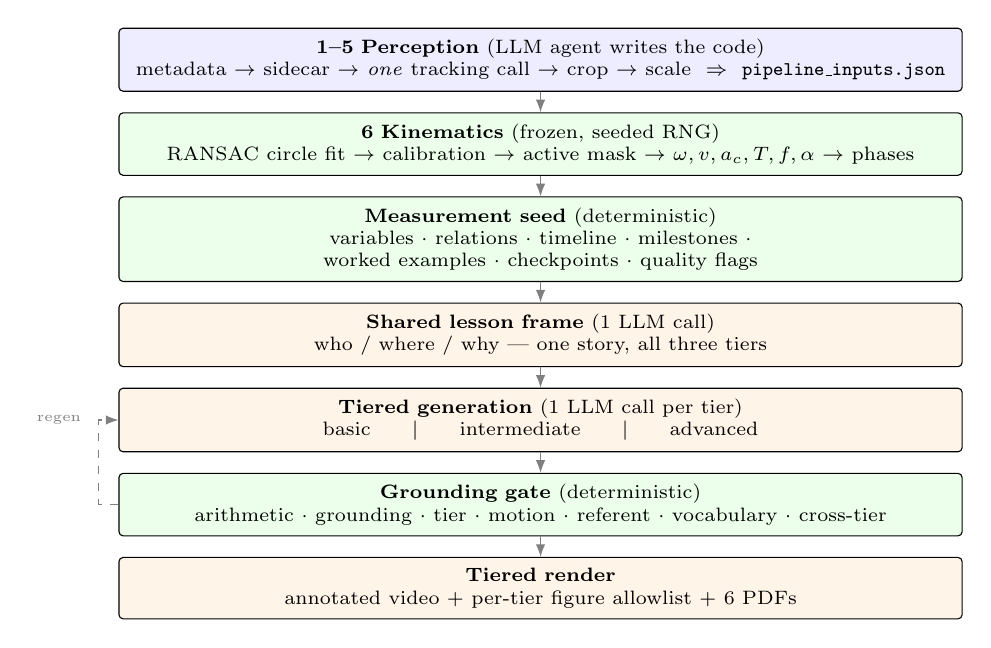
\begin{tikzpicture}[
  node distance=2.6mm,
  box/.style={draw, rounded corners=1.5pt, align=center, font=\scriptsize,
              minimum height=5mm, text width=0.86\columnwidth, inner sep=1.4mm},
  agent/.style={box, fill=blue!7},
  frozen/.style={box, fill=green!8},
  gen/.style={box, fill=orange!9},
  arr/.style={-{Latex[length=1.6mm]}, gray}
]
\node[agent] (a) {\textbf{1--5 Perception} (LLM agent writes the code)\\
  metadata $\rightarrow$ sidecar $\rightarrow$ \emph{one} tracking call
  $\rightarrow$ crop $\rightarrow$ scale $\;\Rightarrow\;$
  \texttt{pipeline\_inputs.json}};
\node[frozen, below=of a] (b) {\textbf{6 Kinematics} (frozen, seeded RNG)\\
  RANSAC circle fit $\rightarrow$ calibration $\rightarrow$ active mask
  $\rightarrow$ $\omega, v, \ac, T, f, \alpha$ $\rightarrow$ phases};
\node[frozen, below=of b] (c) {\textbf{Measurement seed} (deterministic)\\
  variables $\cdot$ relations $\cdot$ timeline $\cdot$ milestones $\cdot$
  worked examples $\cdot$ checkpoints $\cdot$ quality flags};
\node[gen, below=of c] (d) {\textbf{Shared lesson frame} (1 LLM call)\\
  who / where / why --- one story, all three tiers};
\node[gen, below=of d] (e) {\textbf{Tiered generation} (1 LLM call per tier)\\
  basic $\;\vert\;$ intermediate $\;\vert\;$ advanced};
\node[frozen, below=of e] (f) {\textbf{Grounding gate} (deterministic)\\
  arithmetic $\cdot$ grounding $\cdot$ tier $\cdot$ motion $\cdot$ referent
  $\cdot$ vocabulary $\cdot$ cross-tier};
\node[gen, below=of f] (g) {\textbf{Tiered render}\\
  annotated video $+$ per-tier figure allowlist $+$ 6 PDFs};
\draw[arr] (a) -- (b); \draw[arr] (b) -- (c); \draw[arr] (c) -- (d);
\draw[arr] (d) -- (e); \draw[arr] (e) -- (f); \draw[arr] (f) -- (g);
\draw[arr, dashed] (f.west) -- ++(-2.5mm,0) |- (e.west)
  node[midway, left, font=\tiny, xshift=-1mm] {regen};
\end{tikzpicture}
\caption{The pipeline. Blue is LLM-authored code executed at run time, green is
frozen deterministic code, orange is an LLM-authored artifact. The measurement
seed is the only channel between the two halves; the dashed edge is the
failure-informed regeneration loop of Alg.~\ref{alg:gen}.}
\label{fig:pipeline}
\end{figure}

\subsection{Capture and the scene sidecar}

The sidecar carries the three things the pixels cannot supply: a
natural-language cue naming the object to track, a reference object with its
real-world size in metres (which sets the pixel-to-metre scale), and the user's
mark for the rotation axis as a fraction of frame width and height.

Cue wording dominates tracking reliability more than we expected: a bare noun
reached $100\%$ tracked-frame coverage on one clip where a colour-modified noun
reached $6\%$. The failure modes are asymmetric---bare nouns fail by returning
nothing, which shows up as a gap, whereas colour cues fail by returning a
whole-frame box, which looks like perfect coverage. Coverage and correctness are
therefore reported separately.

\subsection{Agentic perception (Steps 1--5)}

Fig.~\ref{fig:pipeline} lists the stages. Four rules constrain the agent, all
enforced by the orchestrator prompt rather than by code, and all of them exist
because they were violated at least once:

\begin{enumerate}
\item \textbf{Exactly one tracking call per job}, made on the original video
and cached; crop-space trajectories are derived by subtracting the crop offset,
never by a second call.
\item \textbf{Never fabricate a measurement.} Missing detections become
\texttt{NaN}; a last-known position may not be repeated to fill a gap.
\item \textbf{One coordinate space.} The display-to-crop transform is applied
once, by the frozen code, to the trajectory and the centre together. Splitting
it across two places once put a clip's trajectory $232$~px from its own centre.
\item \textbf{The frozen package is off limits} to the agent.
\end{enumerate}

Three tracking back-ends share one cached output format, selected by the
sidecar, and \textbf{they do not all measure the same thing}
(Table~\ref{tab:modes}). A promptable segmentation-and-tracking
model~\cite{sam} follows a general object; classical HSV colour tracking
follows a marked one; and a blade-pass FFT mode handles objects whose blades
are mutually indistinguishable, where no individual point can be followed at
all. Only the first is a learned detector.

\textbf{The third mode recovers a rate and \emph{synthesises} an orbit from
it.} There is no tracked point, so its trajectory is a construction, and the
figures drawn from it depict a model rather than a measurement. It also has a
floor below which it reports motion that is not there. Two clips were in this
mode; both have been re-shot with a marker, and \textbf{no clip in the reported
corpus uses it.} We describe the mode because the system still implements it,
because the failure it exhibits is instructive, and because measuring that
failure is one of this paper's results rather than a limitation of it.

\label{sec:tracking}
\begin{table}[t]
\caption{Tracking mode by clip. The corpus is not homogeneous, and the third
mode does not produce a measured trajectory.}
\label{tab:modes}
\centering
\footnotesize
\begin{tabular}{@{}p{0.22\columnwidth}p{0.30\columnwidth}p{0.32\columnwidth}@{}}
\toprule
\textbf{Mode} & \textbf{Clips} & \textbf{What is measured} \\
\midrule
Promptable tracker & roundabout, 2 turntables (\textbf{3}) & trajectory, per frame \\
\addlinespace[2pt]
HSV colour & computer fan, ceiling fan (\textbf{2}) & trajectory, per frame \\
\addlinespace[2pt]
Blade-pass FFT & \emph{none --- both clips re-shot} (\textbf{0}) & \emph{was: rate only, orbit synthesised} \\
\bottomrule
\end{tabular}
\end{table}

\textbf{The third mode no longer appears in the corpus, and removing it is a
result.} The two clips that used it were re-shot with a yellow card taped along
one blade, which is enough to track by colour; the re-shot clip reaches
$99.99\%$ coverage over $190.8$ revolutions with no step above eight times its
own median. On its stationary tail the marker track reads $0.016$~rad/s while a
blade-pass FFT over the \emph{same frames} reports $4.69$~rad/s---the mode's
rate floor, measured directly against a method that gets it right, rather than
asserted from its construction. One piece of card converted two synthesised
orbits into one measured trajectory, which is the cheapest fidelity improvement
we found anywhere in this work.

\subsection{Frozen kinematics (Step 6)}

The frozen package cleans, calibrates and differentiates once. A RANSAC circle
fit drawing from a seeded RNG gives an identical fit every run, and the user's
axis mark is overridden only when the fit is unambiguously better on two
independent criteria---so a good mark is never overruled and a mark placed on
the wrong feature is. Angular velocity is computed \emph{once} and that same
series is reused for the active mask, the summary, the period and the phase
segmentation, which is what stops two parts of a document quoting different
values. Speed and centripetal acceleration use the \emph{fitted} radius rather
than the mean of per-frame distances, so $v = \omega r$ and
$\ac = \omega^{2} r$ close exactly at every instant---a property the gate later
depends on. Idle intervals are excluded from every summary statistic: every clip
in the corpus ends at rest, and the at-rest tail has faked a result three times
in this project's history.

One choice is worth the space. \emph{Motion type is fitted, not thresholded.}
Whether a clip is spinning up, coasting down or steady is decided by fitting
$\theta(t)$ over the longest active run to a line versus a parabola and
requiring both a large residual-variance drop and an appreciable change in rate.
Fitting an integral is robust where differentiating and thresholding is not: the
threshold version flickered, and once labelled a clean spin-up as steady.

\subsection{The measurement seed}
\label{sec:seed}

The seed is the only channel between measurement and generation. The generator
never sees the video, the tracker output, or the per-frame series.
Table~\ref{tab:seed} lists what it carries.

\begin{table}[t]
\caption{The measurement seed: the sole input to generation.}
\label{tab:seed}
\centering
\footnotesize
\begin{tabular}{@{}p{0.26\columnwidth}p{0.66\columnwidth}@{}}
\toprule
\textbf{Block} & \textbf{Contents} \\
\midrule
\texttt{variables} & $r$, $\omega$, $v$, $\ac$, $T$, $f$ --- each with value, unit, and a plain-language definition \\
\texttt{relations} & $\omega = d\theta/dt$; $v = \omega r$; $\ac = v^{2}/r = \omega^{2} r$; $T = 2\pi/\omega = 1/f$, each with a plain-language gloss \\
\texttt{angular\_} \texttt{acceleration} & motion type, $\alpha$, $\at = \alpha r$, endpoint rates, resolved \emph{along the direction of travel} \\
\texttt{timeline} & four sampled instants at which the relations close exactly \\
\texttt{angle\_} \texttt{milestones} & times at which the object has swept $90^{\circ}$, $180^{\circ}$, $270^{\circ}$, $360^{\circ}$ \\
\texttt{measurement\_} \texttt{quality} & whether per-instant values are trustworthy on this clip \\
\texttt{narrative\_} \texttt{context} & the scene description supplied at capture \\
\midrule
\multicolumn{2}{@{}l}{\emph{Deterministic pedagogy blocks --- computed, never written by a model:}} \\
& worked examples (faded at advanced), check-your-understanding items, predict-before-reveal prompts, named misconceptions, a transfer prompt on a different object, a self-placement block, per-tier graded steps with checkpoints, an honesty note, and teacher-only notes \\
\bottomrule
\end{tabular}
\end{table}

Two conventions in the seed do disproportionate work. First, there is
\textbf{one canonical angular velocity} that the prose, the summary table and
the figures all quote, and it is a \emph{magnitude}: direction lives in a
separate rotation-direction field. This exists because a signed value quoted in
prose beside an unsigned one in a table produced a passage asserting
$-2.12$ and $2.08$ for the same quantity. Second, every reader-facing dynamic
quantity is resolved \textbf{along the direction of travel}: $\alpha$ is
$d|\omega|/dt$, so negative always means slowing regardless of which way the
object turns, and the endpoint rates are speeds. Taking the sign from the raw
fit instead once produced a basic worksheet that taught ``speeding up'' over a
graph showing a fan slowing down, on both counter-clockwise clips.

\subsection{Difficulty tiering}
\label{sec:tiers}

Difficulty is defined by two measures that must agree: element interactivity
from Cognitive Load Theory~\cite{sweller} (how many quantities and relations
the passage integrates at once) and the Bloom objective~\cite{bloom} the
passage equips the reader to reach. Crucially, a tier is implemented as a
\textbf{restriction on the seed}, not as an instruction to write harder
(Table~\ref{tab:tiers}).

\begin{table}[t]
\caption{Tiers are restrictions on the measurement seed.}
\label{tab:tiers}
\centering
\footnotesize
\begin{tabular}{@{}p{0.13\columnwidth}p{0.36\columnwidth}p{0.16\columnwidth}p{0.17\columnwidth}@{}}
\toprule
\textbf{Tier} & \textbf{Seed fields unlocked} & \textbf{Interactivity} & \textbf{Bloom target} \\
\midrule
Basic & object, direction, duration, $r$, $T$ in seconds, turns per second, the angle milestones, the \emph{idea} of an inward pull & low & Remember / Understand \\
\addlinespace[2pt]
Inter\-mediate & $+\ \omega, \ac, T, f$ with values; $\ac = \omega^{2}r$, $T = 2\pi/\omega = 1/f$ & moderate & Apply / Analyze \\
\addlinespace[2pt]
Advanced & $+\ \alpha$, $\at = \alpha r$, the phase timeline, $\ac \propto \omega^{2}$, the calibration caveat & high & Analyze / Evaluate \\
\bottomrule
\end{tabular}
\end{table}

Three further things vary by tier, and all three must stay synchronised across
the generator, the gate and the renderer or the material contradicts itself.

\emph{Section order.} All tiers share five section headings. Basic prepends a
sixth, \emph{What these words mean}, so terms are defined before the scenario.
Intermediate \emph{reorders} the shared five so the reader interprets the graph
in words \emph{before} meeting the equation---the formula then arrives as the
compact way to say something already seen.

\emph{Worked instants.} Each tier is assigned distinct indices into the seed's
four-instant timeline, so the advanced tier cannot verify its relations at the
same moment the intermediate tier already used. Without this, advanced and
intermediate converge into near-duplicates. Basic is assigned none, because it
performs no numeric verification at all. All of them are skipped when the
measurement-quality flag says per-instant values are untrustworthy.

\emph{Figures.} A basic passage that strips to one variable but is printed
beside an angular-velocity graph, a quadratic $\ac(t)$ curve and a
thirteen-row table reintroduces exactly the load the prose removed. Each tier
therefore carries a figure allowlist: basic gets a simplified annotated frame
labelled in words, an angle-at-time picture with dots at each milestone, and a
plain traced path, and \emph{no table}; intermediate and advanced add the
time-series plots and a core or full measurements table. The generator is told
its allowlist and the renderer embeds that same list, because a version in
which only one of the two changed produced basic prose describing ``graphs
showing speed and acceleration climbing''---plots the basic tier no longer
showed.

Because a passage the reader merely reads performs no task, the material also
carries deterministic interaction, drawn from the seed blocks in
Table~\ref{tab:seed}: a prediction demanded before any measurement is revealed,
a checkpoint closing each of three graded steps, the documented misconceptions
named and asked about, a transfer prompt on a different object, a
self-placement block, and---at advanced---worked examples that \emph{fade}, the
first worked in full and later ones stopping before the last step. Every answer
is withheld to the teacher edition.

\subsection{Prompt construction}
\label{sec:prompt}

Generation is not one prompt. A system message is assembled per clip and per
tier from a fixed template plus six policy blocks whose content depends on what
was actually measured (Table~\ref{tab:prompt}). This is where most of the
system's pedagogical control lives, and it is the part a reader trying to
reproduce the work would need.

\begin{table}[t]
\caption{What the per-tier system prompt is assembled from. The nine hard rules
are constant; the six policy blocks are computed per clip from the seed.}
\label{tab:prompt}
\centering
\footnotesize
\begin{tabular}{@{}p{0.24\columnwidth}p{0.68\columnwidth}@{}}
\toprule
\textbf{Component} & \textbf{Content} \\
\midrule
Tier header & the Bloom target, the interactivity target, the unlocked seed fields, the forbidden list, and the figure allowlist for \emph{this} tier \\
\addlinespace[2pt]
Rules 1--2 & numbers only from the data, quoted to three significant figures, and \emph{never re-derived}: a measured $T$ must be printed as measured, not recomputed from $2\pi/\omega$. Exposition only --- no questions \\
Rule 4 & verify a relation at a \emph{single} timeline instant, where $v = \omega r$ and $\ac = \omega^{2}r$ close exactly, never with summary means \\
Rule 5 & narrate only figures on this tier's allowlist \\
Rule 6 & interactivity and Bloom must point at the same tier; if they disagree, rewrite \\
Rule 8 & teach the physics, not the pipeline: a banned tracking/analysis vocabulary, no figure filenames, figures referred to by what they show \\
Rule 8b & kinematics only --- describe \emph{how} it moves, never \emph{why}; a banned dynamics vocabulary, so no motor, brake, friction or force \\
Rule 8c & high-school reading level at \emph{every} tier: a banned formal-register vocabulary, with the formal statement re-routed to teacher-only notes \\
Rule 8d & one moment per sentence: never place a lap time from one instant beside a rate from another \\
Rule 9 & plain Unicode, no \LaTeX{} --- a stray backslash makes the reply unparseable \\
\midrule
\multicolumn{2}{@{}l}{\emph{Computed per clip:}} \\
Motion policy & the measured motion type, phrased so the passage cannot contradict it \\
Quality policy & when per-instant values are unreliable, the time-anchored samples are \emph{removed from the prompt entirely} rather than forbidden \\
Anchor policy & this tier's assigned worked instants \\
Steps policy & the three graded steps and their checkpoints \\
Definitions policy & which terms must be defined before use \\
Hints file & per-clip first-pass steering, edited by hand \\
\bottomrule
\end{tabular}
\end{table}

The quality policy deserves emphasis because it is a general lesson. When the
measurement-quality flag marks a clip's per-instant values untrustworthy, the
system does not tell the model not to use them---it \emph{deletes the
time-anchored samples from the prompt}. Removing the temptation proved far more
reliable than forbidding its use.

The output is constrained to a JSON object with an exact, tier-dependent set of
section keys, plus self-reported Bloom objective, element interactivity, and
concepts used. Three identity fields---scene title, object name, and tier---are
\emph{overwritten} after parsing rather than trusted, so a tier cannot invent
its own title and cannot mislabel its own level.

\subsection{The generation loop}
\label{sec:loop}

All generation uses \texttt{Qwen3.6-35B-A3B} (a sparse mixture-of-experts model
with $\approx$3\,B active parameters, 4-bit quantised), served locally over an
OpenAI-compatible endpoint at temperature $0.4$ with a $24{,}000$-token
completion budget; the shared-frame call and the judge runs of
Sec.~\ref{sec:evaldesign} use temperature $0$. Output is parsed as JSON with a
fixed, tier-dependent key set.

Generation runs one call for a shared \emph{lesson frame} (who, where, why: one
story reused by all three tiers so they describe the same situation), then one
call per tier, then a bounded repair loop (Alg.~\ref{alg:gen}).

\begin{algorithm}[t]
\caption{Tiered generation with failure-informed repair}
\label{alg:gen}
\footnotesize
\begin{algorithmic}[1]
\State $\textit{frame} \gets \Call{GenFrame}{\textit{seed}}$
\Comment{one shared story}
\ForAll{$t \in \{\text{basic}, \text{intermediate}, \text{advanced}\}$}
  \State $\textit{facts} \gets \Call{Restrict}{\textit{seed}, t}$
  \State $m_t \gets \Call{Gen}{t, \textit{facts}, \textit{frame}}$;\;
         $I \gets \Call{Gate}{m_t}$
  \For{$k = 1$ \textbf{to} $2$}
    \If{$I = \emptyset$} \textbf{break} \EndIf
    \State $c \gets \Call{Gen}{t, \textit{facts}, \textit{frame}, I}$
    \Comment{$I$ verbatim}
    \State $J \gets \Call{Gate}{c}$
    \If{$|J| < |I|$} $m_t \gets c$;\; $I \gets J$ \EndIf
    \Comment{strict only}
  \EndFor
\EndFor
\State $X \gets \Call{CrossTier}{m_{\text{basic}}, m_{\text{int}}, m_{\text{adv}}}$
\ForAll{$t \in \Call{Implicated}{X}$}
  \Comment{separate budget, once}
  \State $c \gets \Call{Gen}{t, \cdot, \cdot, X_t \cup I_t}$
  \If{$|\Call{Gate}{c}| \le |I_t|$} $m_t \gets c$ \EndIf
\EndFor
\State \textbf{write} all $m_t$ \textbf{and} the gate report
\Comment{never block}
\end{algorithmic}
\end{algorithm}

Four properties of this loop are load-bearing.

\emph{Repair is failure-informed, not blind.} A re-roll at the same temperature
rarely clears the same fault on its own. The retry receives the gate's exact
issue strings, each of which already names the offending phrase or number, and
is told to change nothing else.

\emph{A re-roll is kept only on strict improvement.} Lateral trades are common
and worthless---the model swaps one banned word for another---so a candidate
with an equal issue count is discarded.

\emph{Cross-tier repair has its own budget.} Title equality, distinct worked
instants and rising element interactivity are properties of the \emph{set}, not
of any one passage, so a tier that has spent its per-tier retries can still be
repaired once for cross-tier fit.

\emph{The pipeline never hard-blocks on prose.} All three passages are written
with their issues recorded beside them in a machine-readable gate report. We
would rather measure the failure rate than hide it; a deployment would have to
revisit this.

On the corpus of Sec.~\ref{sec:evaldesign} the loop terminates with $19$ of
$21$ tiers carrying no issue; the two residuals are a single banned word and a
single ungrounded quantity, one each on two different clips. The two
set-level families fire once each: a cross-tier violation on one clip (an
intermediate tier reusing another tier's worked instant) and a
seed-consistency violation on another (a tabulated period that does not close
against $2\pi/\omega$). Both are recorded rather than repaired away, and the
second is discussed in Sec.~\ref{sec:jumps} because it is a symptom of a
measurement fault rather than a writing fault.

The one failure class this does not fix is a model repeating a banned word when
told to remove it. Our local model drafts well and self-corrects poorly, which
is a documented property of small sparse models: drafting is a forward task,
self-correction is a meta task. The durable lever is therefore first-pass
steering---the hints file and the policy blocks---rather than regeneration. A
generate-$K$-and-select variant, which plays to drafting and around
self-correction, is implemented behind a flag but is not the default.

\subsection{The deterministic grounding gate}
\label{sec:gate}

The gate reads a finished worksheet and returns a list of issue strings. It
contains no model, needs no network, and gives the same answer every time on
the same text. Its rule families are listed in Table~\ref{tab:gate}.

\begin{table}[t]
\caption{Grounding-gate rule families.}
\label{tab:gate}
\centering
\footnotesize
\begin{tabular}{@{}p{0.24\columnwidth}p{0.68\columnwidth}@{}}
\toprule
\textbf{Family} & \textbf{What it refuses} \\
\midrule
Arithmetic closure & a stated product or quotient that does not evaluate, within tolerance, to the stated result \\
Number grounding & any numeral in the prose that does not trace to a seed value or a sanctioned derivation of one \\
Tier compliance & vocabulary, symbols, units and formula use outside the tier's allowance \\
Motion faithfulness & prose whose direction, phase labels, or ``speeding up / slowing down'' disagree with the measurement \\
Referent binding & a rate and a period attributed to the same moment when they come from different moments \\
Vocabulary fences & tracking and pipeline jargon, dynamics vocabulary, formal-register terms, and idioms the reader cannot check \\
Story fence & a framing narrative that smuggles in ungraded physics vocabulary \\
Cross-tier & tiers that share a worked instant, duplicate titles, or fail to separate in element interactivity \\
Annotation & a figure annotation whose value or label does not trace to the seed, checked against the phases that tier's graphs actually draw \\
Seed self-consistency & the deterministic blocks themselves: worked examples and the summary table are checked against the relations \emph{independently of the model} \\
\bottomrule
\end{tabular}
\end{table}

The last family is worth separating out, because it checks the system rather
than the model: it recomputes the deterministic worked examples and the summary
table against the relations, and it is what would have caught a worked example
printing $-4.07$ for an expression equal to $-1.34$, and a table in which
$v \neq \omega r$.

Readability is computed and \emph{reported}, never enforced---see
Sec.~\ref{sec:results} for why optimising it would be a mistake.

\subsection{Tiered rendering and annotation on video}

The renderer emits per-tier figure sets, a core or full measurements table, and
two LaTeX documents per tier (student and teacher). Basic-tier variants are
separate renders, not restyled versions: a simplified annotated frame labelled
in words rather than symbols, an angle-at-time figure whose dots are drawn from
the \emph{same} milestone function the basic prose narrates---so figure and
text agree by construction---and a single-colour traced path with no phase
legend. On a clip flagged for oblique capture the quarter-turn dots are
dropped, leaving only the half and full turn.

Annotation on video is the artifact the parent line does not have in this form.
Rather than one still image with vectors, the system overlays the tracked
object, the fitted orbit, the radius, and labels for $r$, $v$, $\ac$ and
$\omega$ across the whole motion, with a definitions legend. The overlay is
\textbf{symbol-only}: it never prints numeric values, because the student is
meant to measure them rather than read them off.

Direction of travel is drawn from the resolved rotation label, never from the
sign of a stored quantity. That rule exists because it was violated. The fix
that made the stored angular velocity a magnitude (Sec.~\ref{sec:seed})
silently removed the only signal the drawing code was reading, so the direction
test became identically true and both arrows were drawn clockwise on every
clip---wrong on all six worksheets of the two counter-clockwise fan clips. The
separation is now enforced by test: anything needing to know \emph{which way}
reads the direction label, anything needing \emph{how fast} reads a magnitude,
and neither is derived from the other.

% ===========================================================================
\section{Evaluation Design}
\label{sec:evaldesign}
% ===========================================================================

\subsection{Corpus and unit of evaluation}

The corpus is five clips of everyday circular motion: a ceiling fan, a desktop
computer fan, a playground roundabout, and two record-turntable clips. Each
yields three worksheets, so the unit count is $n = 15 = 5 \times 3$, with $5$
per level. Some diagnostics are computed per document section instead, giving
$n = 75 = 15 \times 5$; every figure below counts worksheets unless stated.
Each worksheet ships as a student and a teacher edition, so the rendered corpus
is $30$ English documents, with a parallel Bahasa Indonesia edition for an
Indonesian teacher panel.

\textbf{Three clips were removed during this work, and we report the corpus at
its final size rather than its largest.} Two ceiling-fan clips ran in the
blade-pass mode described in Sec.~\ref{sec:tracking}, which measures a rate and
synthesises an orbit from it; they were re-shot with a marker on one blade so
that the trajectory is measured, and the re-shot clip replaces both. One
turntable clip was withdrawn after its tracked point was found to teleport
(Sec.~\ref{sec:defects}). No result in this paper is computed over the removed
clips, and no number is rescaled from an earlier corpus: every aggregate was
re-derived.

\textbf{The corpus is five clips of roughly four scenes}, not five independent
phenomena: two turntable clips share an object and a setup, and the two fans
differ in size but not in kind. Findings about \emph{between-clip} variation
should be read with that in mind---in particular the low lexical diversity of
the basic tier (Sec.~\ref{sec:results-auto}) may be a property of a narrow
scene set as much as of the generator, and we do not separate the two.

The unit of evaluation is a \emph{learning-material passage with its figures},
not a word problem. This is why rubric rows that presuppose a task---problem
answerability, solvability, variety of solution strategies---are dropped rather
than scored, and it is why the multimodal rubric is scored per tier with
absent modalities marked \texttt{n/a}.

\subsection{The four layers}

\textbf{Layer 0 --- deterministic gate} (Sec.~\ref{sec:gate}). Zero cost, runs
first, produces the ground truth the later layers consume.

\textbf{Layer 1 --- intrinsic difficulty.} Element interactivity, distinct
quantities, relations, Flesch reading ease, Flesch--Kincaid grade~\cite{fk}, and words
per sentence, computed from the finished prose with no model in the loop.

\textbf{Layer 2 --- reference-based similarity.} BERTScore~\cite{bertscore}
F1/R/P, BLEU-4~\cite{bleu}, ROUGE-1/2/L~\cite{rouge} against a single
authentic reference (OpenStax \emph{College Physics}~\cite{openstax} \S6.2, reorganised into our section structure), plus a
reference-free diversity score (one minus mean pairwise cosine similarity of
sentence embeddings). Reported in the layout P-MAGIC~\cite{pmagic} publishes, so
the two sets of numbers can be read side by side.

\textbf{Layer 3 --- LLM-as-a-judge}~\cite{mtbench,geval}. Twelve criteria in
three axes, each scored $1$--$5$, plus an achieved-Bloom label. Eleven criteria are adopted
from the parent line so the rows align with published results; P-MAGIC scores
difficulty directly (their ``difficulty level'', $\kappa = 0.750$) and we keep
it as \emph{difficulty fit}. \textbf{Only grounding accuracy is ours}, and it
exists because neither parent generates from a measurement a passage can be
checked against. Each judge sees one worksheet, the written
rubric, and the measured seed values as reference.

\textbf{Layer 4 --- multimodal judge.} Eleven further criteria scored by a
vision-capable rater that is shown the rendered figures: image--text precision
and relevancy, four text--graph criteria, four text--table criteria, and
annotation correctness on the video frame. Twelve text criteria plus eleven
figure criteria is the full 23-item instrument.

\subsection{Two raters and a frozen prompt}

Layer 3 was run twice, by models from different vendors:
\texttt{Qwen3.6-35B} served locally at temperature $0$---which is also the
model family that \emph{wrote} the material---and \texttt{claude-opus-5}, run
as seven independent blind raters, one per clip, each shown only its own three
worksheets and told nothing about the other run or any existing evaluation.

Both raters were sent the \textbf{byte-identical prompt}. The prompt is
assembled once and written to a file, and each rater is then handed that file
verbatim. This is not ceremony: if two raters are given two separately
assembled prompts, a difference in their scores cannot be attributed to the
judgement rather than to the question, and every agreement figure in
Sec.~\ref{sec:results} depends on that being impossible by construction.

Agreement is reported as Cohen's $\kappa$~\cite{cohen} with \emph{quadratic}
weights~\cite{cohenw}, on the
grounds that scoring 4 where the other rater said 5 is a near miss on an
ordinal scale; the unweighted value is reported beside it. Criteria on which
one rater never varies are reported as \texttt{n/d} rather than $0$, or
``always agreed'' prints as ``never agreed.''

\subsection{Measurement ground truth}

One clip was filmed while the object---a phone lying on a turntable---logged
its own gyroscope, giving $490$ samples at $\approx$60~Hz of the rotation about
the turntable axis. Video and sensor are aligned by scanning the lag that
maximises their correlation, which is robust to the phone having begun logging
before recording started. Magnitudes are compared, so neither leg's sign
convention matters.

\textbf{The sensor bounds one quantity only.} A gyroscope measures angular
rate. It cannot measure the orbit radius or the pixel-to-metre scale, so we
report no sensor comparison for $v$ or $\ac$: a ``gyroscope $\ac$'' would be
$\omega_{\text{gyro}}^{2} r$ computed with \emph{the same} $r$ as the video
leg, the radius would cancel, and the agreement would carry no information
beyond the $\omega$ agreement. \textbf{The metre scale is therefore validated
by nothing in this paper}, and every SI quantity we report inherits that.

% ===========================================================================
\section{Results}
\label{sec:results}
% ===========================================================================

\subsection{Measurement fidelity against a sensor}

We ran the comparison on \emph{two} runs of the same clip, and the difference
between them is the finding (Table~\ref{tab:gyro}). Both consume the identical
video file and the identical sidecar; they differ only in what the agentic half
resolved. One applied a perspective rectification and one did not---\emph{and,
as we establish below, one tracked the marker cleanly and one did not.}

\textbf{This clip has since been withdrawn from the corpus} because its tracked
point teleports (Sec.~\ref{sec:defects}); it contributes no worksheets to any
result in this paper. We retain the sensor comparison because it is the only
external measurement check we have, and because---read correctly---it caught
that defect independently, weeks before the jump sweep did.

\begin{table}[t]
\caption{Measured $|\omega|(t)$ against a phone gyroscope, over the sensor's own
motion window ($n = 461$ resampled instants). Two runs of the \emph{same} video
with the \emph{same} sidecar. Reproduce with
\texttt{tools/gyro\_compare.py}.}
\label{tab:gyro}
\centering
\footnotesize
\begin{tabular}{@{}lcc@{}}
\toprule
& \textbf{as shipped} & \textbf{rectified} \\
\midrule
alignment lag & 1.340 s & 1.210 s \\
alignment $r$ & \textbf{0.720} & \textbf{0.999} \\
\midrule
mean $|\omega|$, video & 5.543 rad/s & 5.822 rad/s \\
mean $|\omega|$, gyroscope & 5.836 rad/s & 5.836 rad/s \\
\quad error & $-5.0\%$ & $\mathbf{-0.2\%}$ \\
\addlinespace[2pt]
peak $|\omega|$, video & 12.348 rad/s & 9.781 rad/s \\
peak $|\omega|$, gyroscope & 9.838 rad/s & 9.842 rad/s \\
\quad error & $\mathbf{+25.5\%}$ & $-0.6\%$ \\
\addlinespace[2pt]
per-instant, RMS & $28.1\%$ & $\mathbf{3.7\%}$ \\
per-instant, median $|$err$|$ & $16.1\%$ & $2.0\%$ \\
\midrule
fitted radius & 0.2037 m & 0.1477 m \\
\bottomrule
\end{tabular}
\end{table}

\textbf{The pipeline can measure angular rate to a few tenths of a percent on
the mean, and it did not do so in the run that produced this paper's corpus.}
The rectified run tracks the sensor at $r = 0.999$ with a mean error of
$-0.2\%$ and a per-instant RMS of $3.7\%$. The shipped run tracks it at
$r = 0.720$, overstates the peak by $25.5\%$, and carries a per-instant RMS of
$28.1\%$. Its mean survives at $-5.0\%$, because the errors are transient and
average out---which is the clearest statement of this system's governing
property we can make.

\textbf{Correction: the peak error is not the rectification.} An earlier draft
read Table~\ref{tab:gyro} as a rectification result, because rectification is
the difference the two runs advertise. It is not the difference that matters
here. The shipped run's tracked marker \emph{teleports}: three frames displace
it by $604$--$713$~px against a median step of $1.44$~px, and the pipeline's
$21$-frame smoothing spreads each into a $\pm12$-frame ramp. Excluding those
frames and recomputing, with \emph{no other change and no rectification}:

\begin{center}
\footnotesize
\begin{tabular}{@{}lcc@{}}
\toprule
& peak $|\omega|$ & error vs sensor \\
\midrule
shipped, all frames & 12.348 rad/s & $+25.5\%$ \\
shipped, teleport frames excluded & 9.431 rad/s & $\mathbf{-4.1\%}$ \\
rectified run & 9.781 rad/s & $-0.6\%$ \\
\midrule
gyroscope & 9.838 rad/s & --- \\
\bottomrule
\end{tabular}
\end{center}

\textbf{Three bad frames out of $350$ account for essentially the whole peak
error}; rectification and the remaining handoff differences account for the
last few points. The rectified run also happens to carry \emph{zero} steps over
$100$~px, so the two effects were confounded in every previous reading of this
table. Separating them was possible only because the sensor gives an external
reference---neither the deterministic checker nor either LLM judge can see a
$3$-frame defect in a trajectory.

\textbf{What this licenses, and what it does not.} It licenses the claim that
the pipeline's rate measurement is sensor-accurate to a few tenths of a percent
on the mean when the tracker behaves. It does \emph{not} license attributing
that accuracy to rectification, and we no longer do. It also demonstrates the
paper's central methodological point on its own most-quoted table: \emph{a
number can be reproducible, traceable and wrong}, and the layer that caught it
was the one with an independent physical reference.

\textbf{Averages are trustworthy and instants are not, by an order of
magnitude.} Even in the good run the mean error ($0.2\%$) is $18\times$ smaller
than the per-instant RMS ($3.7\%$). This is not a defect to be engineered away;
it is a property of differentiating a tracked position, and it is why the tier
rules forbid the basic tier from making per-instant claims at all
(Sec.~\ref{sec:tiers}) and why the seed marks per-instant reliability as a flag
the generator consumes (Sec.~\ref{sec:seed}).

\textbf{The divergence is entirely in the agentic half, and this qualifies the
determinism argument of Sec.~\ref{sec:system}.} The two runs' handoff files
differ in resolved frame rate ($59.769$ vs $59.940$), hub position, reference
extent ($1025$ vs $1078$ px) and crop box---all Step-1--5 outputs, from a
byte-identical sidecar. The frozen half is exactly reproducible and we verified
it; the \emph{delivered measurement} is not, because the perception that feeds
it is not. Freezing the physics bounds one class of variance and leaves another
untouched, and the second class moved the fitted radius by $38\%$ on this clip.
We regard this as the paper's most transferable engineering result: a
determinism boundary is only as strong as the least reproducible stage upstream
of it.

A further consequence lands on Sec.~\ref{sec:jumps}. That section attributes
this clip's inflated $\ac$ to tracker jumps. The rectified run reaches a
comparable value by a different route---a $38\%$ smaller radius---so
rectification and jump rejection may be addressing one error or two. We report
both and separate neither; doing so needs a run that applies both, which we
have not performed.

Seven hypotheses for the residual per-instant error were tested. Five were
rejected outright: the tracker's box quality is not the limit (a structurally
different detector reproduces the same ripple), the box centroid specifically
is not the limit (box orientation, a different observable from the same box,
scores the same), a higher frame rate does not help (error is flat from 15 to
60~fps), the object leaving frame is not the cause, and swapping the smoother
removes $58\%$ of the effect while doubling overall error. One was
\emph{not demonstrable} rather than rejected---no clip's ripple beats its own
surrogate null, which is an absence of evidence and not evidence of
absence---and one, a dropped camera frame, explains $12\%$. About a third of
the effect remains unexplained.

\textbf{This rests on one clip.} Nothing here graduates on a single trace, and
sensor logs for the other six clips are the highest-value missing input in the
project.

\subsection{The gate}

Nineteen of twenty-one worksheets pass every rule the gate carried at the time
of the sweep. The two failures are a banned word (``frame'') in one advanced
worksheet and an ungrounded ``1.8 seconds'' in one intermediate worksheet.

Two cautions attach to that figure. First, \textbf{the generator does not
reproduce}: two runs of the same material over the same corpus scored $21/21$
and $19/21$. Single-run \emph{generation} numbers
must be quoted with the run named or replaced with a mean across runs. Second,
the score is a function of the rule set. Adding the referent-binding rule---
which catches a worksheet stating that a full turn takes $2.07$~s and then
calling $0.30$ turns per second ``\emph{that} turn rate,'' a $3.34$~s
turn---drops the score to $13/21$. Both numbers are real measurements (the
fastest lap and the clip average); the fault is the pronoun, and every number
traces, so the older rule set passed it.

It is worth being precise about how far that rule is corroborated, because our
first reading of it was wrong. Rater~A separates the corpus exactly as the rule
does: the one basic worksheet the rule passes scores $5/5$ on grounding, and
the six it flags score $1, 1, 1, 2, 2, 3$. \textbf{Rater~B does not separate
them at all}---it scores the passed worksheet $4$, ties three of the flagged
six at $4$, and puts three below at $2$. So the agreement is between a
deterministic rule and \emph{the model that also wrote the material}, on the
one criterion the two raters are shown below to agree on least
($\kappa = -0.04$). It is not independent corroboration, and we no longer
present it as such.

Two things follow. The weaker one is that this is the $\kappa$ result appearing
where it matters rather than as a table entry. The stronger one is a rule we
now apply throughout: \textbf{rater~A cannot be relied on for grounding}, and
every grounding conclusion in this paper is drawn from rater~B or from the
deterministic gate.

Attempting to fix the fault by \emph{instruction} made things worse.
Regenerating with an explicit prohibition dropped the gate from $19/21$ to
$16/21$ and the judge mean from $4.12$ to $3.90$ while clearing only $2$ of $6$
instances; that generation was discarded. A prompt rule cannot make a model
careful about a referent. The durable fix is to hand the writer a period and a
rate already paired to the same moment, so the contradiction cannot be written.

\subsection{The difficulty ladder}

The tiers are designed to differ; Table~\ref{tab:ladder} asks what can be
\emph{measured} from the finished prose, and the answer separates cleanly into
one thing that is verified and one thing that is not.

\begin{table}[t]
\caption{Intrinsic measures over the five clips, with what each one licenses.
``Rises'' counts clips on which the measure increases strictly across all three
tiers. $^\dag$Cognitive demand is scored in whole points on a 1--5 scale, so a
per-clip strict rise requires two distinct increments within five levels; both
raters' \emph{means} rise monotonically while individual clips frequently tie.
The strict count is reported for honesty, not as the claim.}
\label{tab:ladder}
\centering
\footnotesize
\begin{tabular}{@{}lccccl@{}}
\toprule
\textbf{Measure} & \textbf{basic} & \textbf{inter.} & \textbf{adv.} & \textbf{Rises} & \textbf{Status} \\
\midrule
Element interactivity & 5.0 & 22.4 & 36.6 & 5/5 & \emph{enforced} \\
Cognitive demand, A & 2.80 & 3.60 & 4.80 & 3/5$^\dag$ & measured \\
Cognitive demand, B & 3.00 & 3.20 & 4.20 & 0/5$^\dag$ & measured \\
\addlinespace[2pt]
Words per sentence & 8.5 & 7.2 & 12.8 & --- & measured \\
Flesch--Kincaid grade & 4.0 & 3.8 & 6.6 & 2/5 & measured \\
Passage length (words) & 469 & 340 & 610 & --- & measured \\
\bottomrule
\end{tabular}
\end{table}

\textbf{Element interactivity rises on 5/5 clips, and that is a conformance
check rather than a finding.} We state this plainly because it would otherwise
read as evidence. Element interactivity here counts the distinct physical
quantities and explicit relations a passage contains; a tier is \emph{defined}
by which quantities and relations the seed unlocks for it
(Table~\ref{tab:tiers}); and the cross-tier gate \emph{fails} any set whose
element interactivity does not rise, which triggers the repair loop of
Alg.~\ref{alg:gen}. So the measure is close to definitional, and where it is
not, the pipeline regenerates until it holds. What 5/5 establishes is that the
generator satisfied its specification on every clip. It does not establish that
a reader would find the tiers harder. The basic tier scores exactly $5.0$ on
every clip in the corpus, which is the clearest statement of how definitional
the measure is: that tier is forbidden equations, so its relation count is
structurally zero and only its quantity count survives.

\textbf{The tier claim therefore rests on cognitive demand, which nothing in the
pipeline enforces.} It is scored by both judges, rises monotonically in the mean for both
($2.80 \rightarrow 3.60 \rightarrow 4.80$ and
$3.00 \rightarrow 3.20 \rightarrow 4.20$), and is the criterion on which the two
raters agree most closely ($\kappa = 0.70$, $r = 0.80$)---the only criterion
whose agreement is strong on a corpus this size. That is independent evidence of the kind element interactivity cannot
supply.

\textbf{Reading grade does not ladder, and we do not claim it}: it rises on two
clips in five, and the intermediate tier reads easiest of the three. This is
not a defect in the material. Flesch--Kincaid sees only sentence length and
syllables per word, so it cannot see an equation---$\ac = \omega^{2}r$ is a
handful of short tokens---and the tier whose difficulty is carried by symbols
therefore scores as the simplest prose. It is a negative result on our own
design claim, and we report it because a difficulty ladder that only appears in
the measure we enforce would not be worth reporting at all.

\subsection{Reference-based similarity}
\label{sec:results-auto}

Table~\ref{tab:auto} gives the automatic layer. Every metric except diversity
compares our text to a single reference, so a high score means \emph{more like
OpenStax}, never \emph{better teaching}.

\begin{table*}[t]
\caption{Reference-based automatic metrics, in P-MAGIC's published
layout~\cite{pmagic}. $n$ counts worksheets. LSTM fluency is P-MAGIC's fifth
metric; it requires their trained weights, which are not published, and is
reported as \texttt{n/a} rather than dropped so that the gap stays visible.}
\label{tab:auto}
\centering
\footnotesize
\begin{tabular}{@{}llcccccccccc@{}}
\toprule
\textbf{Level} & \textbf{n} & \textbf{Stat.} & \textbf{BERT F1} & \textbf{BERT R} & \textbf{BERT P} & \textbf{BLEU-4} & \textbf{ROUGE-1} & \textbf{ROUGE-2} & \textbf{ROUGE-L} & \textbf{Diversity} & \textbf{LSTM} \\
\midrule
basic & 5 & M & 0.799 & 0.790 & 0.808 & 0.019 & 0.270 & 0.038 & 0.132 & 0.185 & n/a \\
 & & SD & 0.002 & 0.004 & 0.002 & 0.008 & 0.017 & 0.007 & 0.008 & --- & n/a \\
\addlinespace[2pt]
intermediate & 5 & M & 0.824 & 0.827 & 0.822 & 0.034 & 0.359 & 0.079 & 0.169 & 0.295 & n/a \\
 & & SD & 0.003 & 0.002 & 0.003 & 0.010 & 0.017 & 0.010 & 0.009 & --- & n/a \\
\addlinespace[2pt]
advanced & 5 & M & 0.828 & 0.828 & 0.828 & 0.035 & 0.404 & 0.095 & 0.176 & 0.316 & n/a \\
 & & SD & 0.003 & 0.004 & 0.002 & 0.010 & 0.014 & 0.009 & 0.007 & --- & n/a \\
\addlinespace[2pt]
\textbf{Total} & 15 & M & \textbf{0.817} & 0.815 & 0.819 & 0.029 & 0.344 & 0.071 & 0.159 & 0.293 & n/a \\
 & & SD & 0.013 & 0.018 & 0.009 & 0.012 & 0.058 & 0.026 & 0.021 & --- & n/a \\
\bottomrule
\end{tabular}
\end{table*}

Three readings are worth stating.

\emph{The seven similarity columns tell one story.} BLEU-4 rises
$0.015 \rightarrow 0.040$ and ROUGE-1 $0.276 \rightarrow 0.411$ across the
levels, in the same direction as BERTScore. The n-gram columns are far lower
than the BERT ones by construction: BLEU-4 at $0.029$ means the text almost
never repeats four of the reference's words in a row, which is what one wants
from generated material that is not copying.

\emph{The metric reads the tier, not the clip.} Within-level spread is
$\pm0.003$; across all 21 it is $\pm0.014$. Almost all the variance is between
levels rather than between videos.

\emph{The basic tier is the most formulaic.} Its diversity is $0.185$ against
$0.295$ and $0.316$: the five beginner worksheets resemble each other
considerably more than the harder ones do. Making the beginner text simple has
also made it repetitive. This is a genuine weakness and it is the first
measurement in the project that exposes it.

Finally, the ordering---basic lowest, advanced highest---is not a quality
ranking, because the reference is a college textbook and making the beginner
level more readable therefore lowers its score. Changing the reference text
moves the number by $0.04$, roughly eight times what an entire pedagogy rework
moved it. Report it; do not optimise it.

\subsection{LLM judge and inter-rater reliability}

Table~\ref{tab:judge} gives both raters on all twelve criteria with the
weighted $\kappa$ between them.

\begin{table*}[t]
\caption{Two independent LLM raters on the same 12-criterion rubric and the
byte-identical prompt. Cell entries are M \scriptsize(SD)\normalsize\ over the
five clips at that level; \textbf{N} is the number of scores each cell
averages. $\kappa$ is quadratic-weighted and is computed on a \emph{different}
denominator---all $15$ paired ratings for a criterion row, all $180$ for the
final row---so it should not be read against the N beside it.}
\label{tab:judge}
\centering
\footnotesize
\begin{tabular}{@{}l c c cc cc cc@{}}
\toprule
& \textbf{Cohen's} & & \multicolumn{2}{c}{\textbf{basic}} & \multicolumn{2}{c}{\textbf{intermediate}} & \multicolumn{2}{c}{\textbf{advanced}} \\
\cmidrule(lr){4-5}\cmidrule(lr){6-7}\cmidrule(lr){8-9}
\textbf{Criterion} & $\boldsymbol{\kappa}$ & \textbf{N} & \textbf{Qwen 35B} & \textbf{Claude} & \textbf{Qwen 35B} & \textbf{Claude} & \textbf{Qwen 35B} & \textbf{Claude} \\
\midrule
\multicolumn{9}{@{}l}{\emph{Linguistic / authenticity}} \\
\quad Motivating context & \textbf{--0.04} & 5 & 3.60 \tiny(0.49) & 3.20 \tiny(0.40) & 3.60 \tiny(0.49) & 3.20 \tiny(0.40) & 4.00 \tiny(0.00) & 3.20 \tiny(0.40) \\
\quad Language clarity & 0.19 & 5 & 4.40 \tiny(0.49) & 4.20 \tiny(0.40) & 4.00 \tiny(0.63) & 4.00 \tiny(0.00) & 4.20 \tiny(0.40) & 4.20 \tiny(0.40) \\
\quad Cognitive demand & \textbf{0.70} & 5 & 2.80 \tiny(0.40) & 3.00 \tiny(0.00) & 3.60 \tiny(0.49) & 3.20 \tiny(0.40) & 4.80 \tiny(0.40) & 4.20 \tiny(0.40) \\
\quad Fluency & 0.41 & 5 & 4.40 \tiny(0.49) & 3.80 \tiny(0.40) & 4.20 \tiny(0.75) & 3.40 \tiny(0.49) & 4.80 \tiny(0.40) & 4.00 \tiny(0.63) \\
\quad Completeness & 0.58 & 5 & 3.40 \tiny(0.49) & 3.80 \tiny(0.40) & 4.00 \tiny(0.63) & 3.60 \tiny(0.49) & 5.00 \tiny(0.00) & 4.80 \tiny(0.40) \\
\addlinespace[1pt]
\quad\textbf{axis mean} & --- & 25 & \textbf{3.72} & \textbf{3.60} & \textbf{3.88} & \textbf{3.48} & \textbf{4.56} & \textbf{4.08} \\
\addlinespace[3pt]
\multicolumn{9}{@{}l}{\emph{Structural / comprehension}} \\
\quad Comprehension & 0.18 & 5 & 4.40 \tiny(0.49) & 3.80 \tiny(0.75) & 4.40 \tiny(0.49) & 3.60 \tiny(0.49) & 4.80 \tiny(0.40) & 4.00 \tiny(0.63) \\
\quad Structure clarity & 0.20 & 5 & 4.40 \tiny(0.49) & 4.00 \tiny(0.00) & 4.40 \tiny(0.49) & 3.60 \tiny(0.49) & 4.80 \tiny(0.40) & 3.80 \tiny(0.75) \\
\quad Concept accuracy & 0.14 & 5 & 2.80 \tiny(0.75) & 3.60 \tiny(0.49) & 3.20 \tiny(1.47) & 3.80 \tiny(0.40) & 4.60 \tiny(0.49) & 4.20 \tiny(0.40) \\
\quad Realistic & 0.29 & 5 & 3.40 \tiny(1.20) & 4.20 \tiny(0.40) & 3.80 \tiny(0.98) & 4.20 \tiny(0.40) & 4.60 \tiny(0.80) & 4.20 \tiny(0.40) \\
\quad Variable-name consistency & 0.51 & 5 & 3.60 \tiny(0.80) & 3.60 \tiny(0.49) & 4.20 \tiny(0.75) & 4.40 \tiny(0.49) & 5.00 \tiny(0.00) & 5.00 \tiny(0.00) \\
\addlinespace[1pt]
\quad\textbf{axis mean} & --- & 25 & \textbf{3.72} & \textbf{3.84} & \textbf{4.00} & \textbf{3.92} & \textbf{4.76} & \textbf{4.24} \\
\addlinespace[3pt]
\multicolumn{9}{@{}l}{\emph{Physics / tier}} \\
\quad Difficulty fit & 0.19 & 5 & 4.20 \tiny(0.40) & 4.20 \tiny(0.40) & 4.00 \tiny(0.89) & 4.20 \tiny(0.40) & 4.40 \tiny(1.20) & 5.00 \tiny(0.00) \\
\quad Grounding accuracy & \textbf{--0.07} & 5 & 1.40 \tiny(0.49) & 3.20 \tiny(0.75) & 2.60 \tiny(1.96) & 3.40 \tiny(0.80) & 4.00 \tiny(1.26) & 3.60 \tiny(0.49) \\
\addlinespace[1pt]
\quad\textbf{axis mean} & --- & 10 & \textbf{2.80} & \textbf{3.70} & \textbf{3.30} & \textbf{3.80} & \textbf{4.20} & \textbf{4.30} \\
\addlinespace[3pt]
\midrule
\textbf{All 12 criteria} & \textbf{0.31} & 60 & \textbf{3.57} & \textbf{3.72} & \textbf{3.83} & \textbf{3.72} & \textbf{4.58} & \textbf{4.18} \\
\bottomrule
\end{tabular}
\end{table*}

\textbf{The ordering reproduces; the score does not.} Both raters put advanced
clearly top. Beyond that the agreement thins: the second rater separates basic
from intermediate not at all (both $3.72$), where the first separates them by
$0.26$. The per-level gap between raters is not constant either
($+0.15$, $-0.12$, $-0.40$), so we cannot describe the difference as a simple
calibration offset---an account an earlier draft gave on a previous corpus and
which does not survive re-derivation. Over all $180$ paired ratings the two give
the identical integer $40\%$ of the time and land within one point $88\%$ of the
time. Overall $\kappa = 0.31$ weighted, $0.14$ unweighted.

Two caveats govern how far these may be pushed. \textbf{The overall figure rests
on $180$ pairs; the per-criterion figures rest on $15$ each and are indicative
only}, with intervals wide enough that no per-criterion value should be read as
a point estimate. And \textbf{the corpus is five clips of roughly four scenes},
so between-clip variation is not independent.

The criterion that carries the tier claim is \emph{cognitive demand}:
$2.80 \rightarrow 3.60 \rightarrow 4.80$ for the first rater and
$3.00 \rightarrow 3.20 \rightarrow 4.20$ for the second. It rises in the mean
for both and it is the criterion on which they agree most closely
($\kappa = 0.70$, $r = 0.80$)---by a clear margin over every other row.

\textbf{The criterion a physics worksheet most needs is the one with no
agreement at all.} On grounding accuracy $\kappa = -0.07$, and the raw
agreement is more striking than the coefficient: across fifteen worksheets the
two raters chose the same integer \textbf{zero times}, and landed within one
point on only $33\%$ against $88\%$ overall. Their means now differ as well
($2.67$ against $3.40$), so unlike on our earlier corpus a mean-only comparison
would not have hidden the problem---but it would have understated it.

The cause is diagnosable and is a property of the criterion, not of either
rater. It silently asks two questions---do the numbers trace back to the
measurement, and do the relations printed beside them close?---which come apart
whenever a worksheet correctly reports two measured averages that do not satisfy
the formula linking them. That is common here, because the average of squares is
not the square of the average. One rater penalises a relation that does not
close; the other accepts a faithful report of what was measured. Both readings
are defensible, which is exactly why a single number from a single judge should
not be quoted as a quality score, and why we split this criterion before the
human panel rather than after.

\textbf{Rater A cannot be trusted on this criterion, and the sharpest evidence
is on the current corpus.} On \texttt{turntable-2} the intermediate worksheet
walks the reader through $\ac = \omega^{2}r$ and prints the product as
$4.91$~m/s$^{2}$; the arithmetic gives $4.83^{2} \times 0.185 = 4.31$, a
$13.7\%$ discrepancy, and the passage then asserts the result agrees with the
measured average. Rater~A scored that worksheet $5/5$ on grounding accuracy.
Rater~B scored it $2$ and named the defect. Rater~A is the model that
\emph{wrote} the material, and this is the criterion on which it is being asked
to audit itself.

\textbf{The judge is also wrong in the other direction, and we report both.} On
an earlier corpus rater~A marked a worksheet down for writing
$8.04^{2} \times 0.438 = 28.3$, which is correct to three significant figures.
That is the rater's own arithmetic failing, and it is the reason a model should
not be used to audit sums---a deterministic checker does that better and for
nothing. The judge layer earns its place by catching what a checker cannot ask
about, not by being more reliable than one.

\textbf{A control separates rater difference from run noise.} Re-running the
local judge on the frozen prompts two days after an earlier run reproduced it
exactly: every worksheet, every rating identical, $\kappa = 1.00$. The
judge is deterministic and the gap between raters is real. Set against this the
\emph{writer}, which does not reproduce at all. \textbf{The model that grades is
stable; the model that writes is not.}

\subsection{The multimodal axis}

Table~\ref{tab:axis4} scores the figures. It was run by the vision-capable
rater on the current renders; every previous multimodal score in the project
described figures that no longer exist.

\begin{table}[t]
\caption{Multimodal rubric, single vision-capable rater, M \scriptsize(SD)\normalsize.
\texttt{n/a} marks a modality a tier does not ship.}
\label{tab:axis4}
\centering
\footnotesize
\begin{tabular}{@{}lccc@{}}
\toprule
\textbf{Modality / criterion} & \textbf{basic} & \textbf{inter.} & \textbf{adv.} \\
\midrule
\multicolumn{4}{@{}l}{\emph{Image--text}} \\
\quad Precision & 2.86 \tiny(0.64) & 2.43 \tiny(0.73) & 3.14 \tiny(0.83) \\
\quad Relevancy & 4.57 \tiny(0.49) & 4.57 \tiny(0.49) & 4.57 \tiny(0.49) \\
\quad\textbf{mean} & \textbf{3.71} & \textbf{3.50} & \textbf{3.86} \\
\addlinespace[2pt]
\multicolumn{4}{@{}l}{\emph{Text--graph}} \\
\quad Accuracy \& labelling & 3.43 \tiny(0.73) & 3.29 \tiny(0.45) & 3.14 \tiny(0.64) \\
\quad Scale \& proportions & 4.14 \tiny(0.35) & 4.14 \tiny(0.64) & 3.86 \tiny(0.64) \\
\quad Physical sense & 2.71 \tiny(1.16) & 2.29 \tiny(0.88) & 2.71 \tiny(1.16) \\
\quad Relevancy & 3.14 \tiny(0.83) & 2.86 \tiny(0.64) & 3.29 \tiny(0.88) \\
\quad\textbf{mean} & \textbf{3.36} & \textbf{3.14} & \textbf{3.25} \\
\addlinespace[2pt]
\multicolumn{4}{@{}l}{\emph{Text--table}} \\
\quad Labels \& scales & n/a & 3.29 \tiny(0.45) & 3.29 \tiny(0.45) \\
\quad Proportional reasoning & n/a & 2.29 \tiny(0.45) & 2.57 \tiny(0.49) \\
\quad Physics connection & n/a & 3.71 \tiny(0.45) & 3.86 \tiny(0.35) \\
\quad Relevancy & n/a & 4.14 \tiny(0.35) & 3.29 \tiny(0.70) \\
\quad\textbf{mean} & n/a & \textbf{3.36} & \textbf{3.25} \\
\addlinespace[2pt]
\multicolumn{4}{@{}l}{\emph{On video}} \\
\quad \textbf{Annotation correctness} & \textbf{4.29} \tiny(0.70) & \textbf{4.43} \tiny(0.73) & \textbf{4.29} \tiny(0.70) \\
\midrule
\textbf{All criteria scored} & 3.59 & 3.40 & 3.45 \\
\bottomrule
\end{tabular}
\end{table}

Two results stand out.

\textbf{Annotation correctness is the highest-scoring row in the evaluation}
($4.29$--$4.43$), and it needs two qualifications before it can be used.

\emph{It was scored on still frames, not on the video.} The rater was shown the
rendered annotated \emph{image} for each tier; the annotated video was never
submitted to it. So this row is evidence about frame annotation---which the
parent line also produces---and \textbf{not} about annotation across the
motion, which is the thing that differentiates the system. We therefore do not
cite it in support of the video-annotation contribution. What does support that
contribution is deterministic rather than judged: the figure verifier is clean
on every clip in the corpus, and the direction rule and phase labels described
in Sec.~\ref{sec:system} are pinned by unit tests.

\emph{It is scored against the seed.} The criterion asks whether an overlay
reports the measured value, so an annotation that faithfully draws a
contaminated measurement scores full marks. On the clip discussed in
Sec.~\ref{sec:jumps} it does exactly that. This is the same limit we identify
for the deterministic gate, applied to our own strongest row: \textbf{tracing a
number is not validating it}, whoever or whatever does the tracing.

\textbf{There is no tier ladder in the figures} ($3.59 / 3.40 / 3.45$). The
same rendering code serves all three tiers, so this is unsurprising, but it
matters for what may be claimed: the difficulty result rests on the prose
alone and cannot be supported by pointing at the figures. The weakest row is
\emph{graph physical sense} ($2.29$--$2.71$), i.e.\ figure-versus-physics
contradiction, which is the subject of the next section.

Marking an absent modality \texttt{n/a} rather than scoring it low is a
methodological point, not a bookkeeping one. The basic tier ships no table by
design; scoring the absence would penalise a tier for being correctly built,
and would make it look worse the more carefully it was designed.

\subsection{What each layer alone would have missed}
\label{sec:defects}
\label{sec:jumps}

The strongest empirical claim we can make about the evaluation design is that
each layer caught a defect the others passed. Table~\ref{tab:defects}
summarises; two cases deserve the detail.

\begin{table}[t]
\caption{Defects found in this study, and which layer found each. Every row is
a defect no other layer detected.}
\label{tab:defects}
\centering
\footnotesize
\begin{tabular}{@{}p{0.30\columnwidth}p{0.20\columnwidth}p{0.36\columnwidth}@{}}
\toprule
\textbf{Defect} & \textbf{Found by} & \textbf{Why the others missed it} \\
\midrule
Ungrounded number; banned vocabulary; non-closing arithmetic & gate (Layer 0) & judges rate these as fluent prose \\
\addlinespace[2pt]
Basic tier is formulaic across clips (diversity $0.185$) & similarity (Layer 2) & invisible within a single worksheet \\
\addlinespace[2pt]
Reading grade does not ladder & intrinsic (Layer 1) & the judge scores the tier it is told \\
\addlinespace[2pt]
Contaminated measurement printed as a fact & judge (Layer 3) & the number \emph{traces}, so the gate passes it \\
\addlinespace[2pt]
Caption contradicting its own curve & multimodal (Layer 4) & no text-only rater can see a figure \\
\addlinespace[2pt]
\textbf{Overlay drawn one crop offset off the object} & \textbf{no layer; author inspection} & \textbf{every check shared the trajectory's own frame of reference} \\
\bottomrule
\end{tabular}
\end{table}

\textbf{The last row is the one that qualifies the claim above.} On the
computer-fan clip, every frame overlay---including the annotated figure
embedded in all three of its worksheets---was drawn $328$~px low, placing the
``centre of rotation'' on a fan blade and running the orbit circle off the fan
onto the desk. No layer reported it. It was found by opening the annotated
video and looking.

The reason is instructive, and it is not that a check was missing. The
trajectory had been left in full-frame coordinates while the overlay was
composited onto the cropped video; the trajectory and the fitted centre were
displaced \emph{together}, so every relative quantity stayed correct---the
orbit radius is within $0.5\%$ of a fit made directly against the video, and
angular velocity is unchanged to thirteen significant digits. Nothing was
numerically wrong. The gate checks that printed values trace to the seed, and
they did. The figure checker was written for exactly this defect class, but it
recomputes the expected plot extent from the kinematics table---which was
itself in the displaced frame, so it compared the error against itself and
passed. The judges scored a predecessor run of the same clip that happened to
be registered correctly.

\textbf{A self-consistent frame of reference cannot be audited from inside
itself}, and all four layers were inside it. The repair is a check that appeals
to something outside the data: a trajectory measured on a cropped video cannot
contain a detection outside that video's own frame, so points beyond the crop
rectangle prove the coordinate space without reference to the centre, the
radius, or any fitted quantity. We report this because it bounds what
Table~\ref{tab:defects} is evidence for. Layers catch defects that are visible
in the quantity each layer inspects; a defect that is consistent in every
quantity and wrong only against the world is not a gap between layers but a
gap beneath all of them.

\textbf{A tracker artifact that the gate could not, in principle, catch.} On
one turntable clip the tracked marker normally moves $1.4$~px between frames;
three times it moves $604$, $614$ and $713$~px in a single $17$~ms frame,
flipping between two positions $728$~px apart (Fig.~\ref{fig:jump}). Because
angular velocity is computed from a centrally smoothed angle, each step is
smeared symmetrically into a ramp, so the artifacts render as smooth mountains
rather than single-frame glitches---in the raw rows the marker is frozen to
within $0.1$~px while $\omega$ climbs from $0$ to $10.2$~rad/s, the filter
anticipating a jump that has not happened yet. One of the three jumps falls
inside the measured window, contaminating $18$ of that clip's $106$ active
samples. Removing them moves the headline number from
$\ac = 7.45$ to $5.85$~m/s$^{2}$: \textbf{the shipped worksheets teach a value
$27\%$ too high.} A sweep of every clip against its \emph{own} local median
step---a fixed pixel threshold is useless, since one clip legitimately travels
$\approx240$~px per frame at peak---found the rest clean apart from one clip
whose jumps are confined to the dead tail. \textbf{This clip has since been
withdrawn from the corpus} and contributes to no result reported here; the
defect is retained in this section because the way it evaded detection is the
finding, not the clip.

\textbf{Our own jump detector could not see these jumps, and that is the more
useful result.} The corpus had already been swept by a gate that bounds the
\emph{angle} swept per frame---adopted precisely because an earlier fixed
pixel bound falsely accused the fastest clip in the corpus. It scored this clip
zero jumps. The teleports are largely \emph{radial}: the marker's orbit radius
runs $244 \rightarrow 687$~px across one of them, and an angular bound is blind
to radial displacement by construction. Their tangential components land at
$85$--$86^{\circ}$ against a $90^{\circ}$ threshold. \textbf{Each bound was
adopted to fix the failure the other one caused}, and a step is suspicious if it
is large in angle \emph{or} large radially, each relative to the clip's own
local median rather than to a constant.

\textbf{The gate's number-grounding rules passed this and could not have done
otherwise}: they verify that every number \emph{traces back to the
measurement}, and $7.45$ does trace. No rule of that shape can ask whether the
measurement itself is sound. \textbf{Tracing a number is not validating it.}
The judge flagged the value; a grounding check and a measurement check answer
different questions, and only the second can be wrong about the world.

The gate was not silent on this clip, and the distinction is worth keeping. Its
\emph{seed self-consistency} family---which recomputes the relations
independently of the generator---did fire, reporting that the tabulated period
of $1.469$~s does not close against $2\pi/\omega = 1.176$~s. That is a symptom
of the same contamination, surfaced deterministically by a rule that
interrogates the measurement rather than the prose. The accurate statement is
therefore narrower than ``the gate could not see it'': \emph{grounding} rules
cannot catch a bad measurement, \emph{closure} rules sometimes can, and here
one did.

The two judges also split on this exact worksheet. The clip's contaminated
value appears in both its intermediate and its advanced worksheet; the local
judge flagged the intermediate one (grounding $2$) and gave the advanced one
full marks ($5$), while the independent rater flagged both, citing arithmetic
that does not close. \textbf{The one worksheet in the corpus whose numbers are
known to be wrong was rated perfectly grounded by one judge and badly grounded
by the other.} A single-rater study reports whichever it happens to draw.

\begin{figure}[t]
\centering
\includegraphics[width=\columnwidth]{jump_tt3.png}
\caption{Tracker jumps on one turntable clip. Normal frame-to-frame step is
$1.4$~px; three steps exceed $600$~px. Central smoothing spreads each into a
symmetric ramp, which is why they appear in $\omega(t)$ as smooth features
rather than spikes.}
\label{fig:jump}
\end{figure}

\textbf{A caption asserting the opposite of its own curve.} Rest bands in the
time-series figures were given a printed caption, ``not turning,'' so that
small jitter inside them would not be misread as motion. But the segmenter
marks some genuinely moving stretches as inactive, so on one clip a band
captioned ``not turning'' contained samples at $24.14$~rad/s. \textbf{Eleven of the corpus's twelve rest bands
carried a caption their own curve contradicted.} The gate was clean throughout,
because it checks that annotations trace to the seed and never asks whether a
band label agrees with the curve beneath it. Only a rater that could see the
image caught it.

The fix is a rule rather than a re-label: the caption is suppressed wherever
the band's samples exceed $5\%$ of the series maximum, while the grey shading
stays, because a colour is not a claim. We record the caveat that this stops a
figure asserting something false without making the underlying segmentation
correct---on one clip the rest band still begins about half a second before the
object stops.

A clean deterministic check is evidence about that check's questions and
nothing more. This one verifies that labelled values trace to the seed; it
never asks whether a caption agrees with the curve beneath it. It took a rater
that could look at the picture.

% ===========================================================================
\section{Discussion}
% ===========================================================================

\subsection{Determinism buys different things in different places}

The project's most reusable result is a division of labour. Perception and
prose are stochastic and are treated as such: the tracking cue, the crop, and
the writing all vary run to run, and we quote no single-run generation number
without naming the run. Physics and verification are frozen and are treated as
such: the same inputs give byte-identical statistics, and the gate gives the
same verdict on the same text every time.

The judge sits awkwardly between the two. It is deterministic in the narrow
sense---re-running our local rater reproduced every one of its ratings---and this
is precisely what makes the inter-rater result interpretable, because the
disagreement cannot be run noise. A judge that is stable and biased is more
dangerous than one that is noisy, because its numbers look repeatable.

\subsection{What an LLM judge is good for here}

On this corpus the judge is usable for \emph{ranking} and not for \emph{level}.
The tier ordering reproduces across two unrelated model families; no absolute
figure does. The common practice of rescaling a $1$--$5$ mean onto a $10$-point
scale to compare against a published human panel inherits the problem twice
over: our overall $4.12/5$ becomes $8.2/10$, which lands inside the
$8.18$--$8.58$ range P-MAGIC's teachers gave~\cite{pmagic}. That coincidence is
worth nothing, twice over. The second rater gives $7.2$, and doubling cannot
make two instruments equivalent; and $8.18$--$8.58$ is P-MAGIC's
\emph{linguistic relevancy} row alone, whose $25$ rows span $1.54$ to $8.99$,
so a twelve-criterion mean is not its counterpart. We report the comparison
only to retire it.

\textbf{Self-preference is the obvious alternative explanation for the offset,
and our data argues against it being the whole story.} Rater~A wrote the
material, and LLM evaluators are known to favour their own
generations~\cite{selfpref}, alongside position and verbosity biases that make
single-rater judging fragile~\cite{fairness,mtbench}. If self-preference drove
the gap it should bite hardest where the writer's failures live. It does not:
on grounding accuracy---the criterion that indicts the writer---rater~A is
\emph{not} more generous ($3.10$ vs $3.14$), and on difficulty fit the two are
identical ($4.48$ vs $4.48$). The large gaps are on fluency ($-1.05$), structure
clarity ($-1.00$) and comprehension ($-0.90$): surface-quality rows, where a
harsher marker is the more parsimonious account.

The qualification is that self-preference shows up precisely where a single
instance matters most. On the one worksheet whose measurement is known to be
wrong, rater~A scored grounding $5$ and rater~B scored $2$. An aggregate that
argues against bias and a single case that exhibits it are not in conflict;
they are the reason we treat rater~A's grounding scores as unusable rather than
merely noisy.

The comparison against human raters on the same instrument is unflattering and
worth stating in full. P-MAGIC's ten teachers reach a per-dimension Cohen's
$\kappa$ between $0.63$ and $0.97$, averaging $0.76$~\cite{pmagic}. Our
\emph{best} criterion, cognitive demand at $0.59$, falls below their
\emph{worst}. Two model raters applying a rubric are not a substitute for two
trained readers applying it, and this is the number that shows it.

We would go further and say the useful output of a judge layer is not a score
but a \emph{disagreement}. The per-criterion $\kappa$ column told us something
no mean could: that the criterion asking whether the numbers hold up is being
read as two different questions. That is a fixable defect in a rubric, and it
was invisible until there were two raters.

\subsection{Implications for the human panel}

The instrument is built and already runs on all $21$ worksheets on the same
criteria and the same scale a teacher panel would use; only the human raters
are missing. One change is required first. The grounding-accuracy criterion
must be split---``do the numbers trace to the measurement?'' and ``do the
relations printed beside them close?''---before teachers score it, or the human
$\kappa$ inherits the same ambiguity and will not be interpretable. The
deterministic gate already separates these two questions; the rubric does not.

% ===========================================================================
\section{Limitations and Threats to Validity}
% ===========================================================================

\textbf{Nothing here measures learning.} Every result in this paper is a
property of the text, the figures, or the measurement behind them. No student
has read this material and no learning gain has been measured. P-MAGIC~\cite{pmagic}
has ten teachers scoring a $22$-criterion rubric; Centri has one expert reader
and two model judges, and a model cannot stand in for either a teacher
or a learner. In fairness to the parent line, P-MAGIC states the same gap: its
own conclusion limits its evidence to expert evaluation of a single physics
topic and names classroom intervention and student learning gains as future
work. Neither system has shown that anybody learns from the generated
material.

\textbf{One rater is not independent of the writer.} The local judge is the
same model family that wrote the material, so its scores are evidence rather
than proof. The second rater is independent of the writer, which is the main
thing it adds beyond a reliability figure.

\textbf{The corpus is small and narrow.} Seven clips of broadly similar
circular motion, all filmed by the developers, none by a teacher or student in
a classroom. The diversity metric is depressed directly by that narrowness, and
the capture protocol has not been tested against uncontrolled footage.

\textbf{The sensor validation rests on one clip}, and that clip is the one with
tracker jumps. Sensor logs for the remaining six are the single highest-value
missing input.

\textbf{One clip's published numbers are wrong.} We report the corpus as it was
scored rather than silently regenerating it, because the defect is part of the
result: it is the case that separates ``the number traces'' from ``the number is
right.'' A jump guard is specified but not built, and nothing in the delivered
pipeline currently rejects a marker that moves five hundred times its usual
step.

\textbf{Known open figure defects.} The dashed line labelled ``clip average''
is in fact the mean over the turning window on every time-series plot; two
basic turns-versus-time graphs contradict their own captions; the measurements
table lists a centripetal acceleration that does not equal $\omega^{2}r$, and
the intermediate tier walks the reader through that multiplication and states
the wrong result; and on three clips the fitted circle sits $9$--$21\%$ of a
radius from the traced points while the basic passage asserts that every point
falls on one circle.

\textbf{The generator is the least reliable component.} A local $35$B model
drafts well and self-corrects poorly: told to remove a banned word it re-emits
it or trades it for another. The durable lever is steering the first pass, not
regeneration, and a generate-$K$-and-select loop is implemented but not yet the
default.

\textbf{Three threats to the judge comparison specifically.} The two raters saw
the corpus differently: rater~A scored all $21$ worksheets in one pass, while
rater~B was run as seven agents seeing three worksheets each, so it could not
calibrate a scale across the corpus. That is a plausible partial cause of the
$-0.5$ offset we attribute to harshness, and we cannot separate the two.
Rater~B's test--retest was never measured, so only one side of the comparison
is pinned as deterministic. And the reference text for the similarity layer was
reorganised by us into our own section structure, which may flatter the
resulting scores; we did not measure the effect of that reorganisation.

\textbf{Reproducibility asymmetry.} Generation does not reproduce and judging
does. Numbers in this paper are labelled accordingly, and we recommend the
same discipline generally: name the run for a single-pass generation figure, or
report a mean across runs.

% ===========================================================================
\section{Conclusion}
% ===========================================================================

Centri generates difficulty-tiered, figure-annotated physics learning material
from ordinary video of an everyday object turning, with the physics frozen and
every number verified against the measurement before rendering. On a five-clip
corpus in which every clip's trajectory is measured rather than modelled, the
tier ladder is carried by cognitive demand---the one judge criterion two
independent raters agree on ($\kappa = 0.70$)---while an element-interactivity
ladder that the pipeline itself enforces is reported as a conformance check and
the reading-grade ladder we once claimed does not exist.

The result we would most like carried forward is methodological. Four
evaluation layers each caught a defect that every other layer passed, including
a measurement artifact that a deterministic grounding check cannot detect by
construction, an arithmetic claim that the same check passed because the number
does trace to the measurement, and a figure caption that no text-only rater can
see. Our own jump detector missed the corpus's worst measurement defect because
each of its two successive bounds was adopted to fix the failure the other one
caused. And two LLM judges on a byte-identical prompt reproduce the ordering of
the tiers while agreeing on nothing at all about whether the numbers hold
up---zero exact agreement, across fifteen worksheets, on the criterion a physics
worksheet most needs. A single judge run yields a number that looks like a
measurement; on this corpus it is a property of the rater.

The next step is the one none of these layers can take: physics teachers
scoring the same twelve criteria, after the grounding criterion has been split
in two.

% ===========================================================================
\section*{Ethics and Artifact Availability}

No human subjects took part in this study; the teacher panel described as
future work has not been run, and will require ethics approval before it is.
The footage is of inanimate objects, filmed by the authors; one clip of a
playground roundabout includes a hand entering frame incidentally and no
identifiable person. Worksheets and rendered figures derived from the footage
were sent to a hosted commercial model for the second rater
(Sec.~\ref{sec:evaldesign}); no other data left the lab.

The frozen-prompt method is the part of this work most likely to be reusable:
prompts are built once, written to disk, and replayed verbatim to every rater,
so a score difference cannot be a question difference. \todo{Add the repository
URL, the frozen prompt set, the judge outputs for both raters, and
\texttt{tools/gyro\_compare.py}, or state why not. The reproduction script for
the two-rater comparison already exists and should be an appendix.}

% ===========================================================================
\section*{Acknowledgment}
\todo{lab, funding, and the sibling-project team}

% ===========================================================================
\noindent\todo{Verify every entry against the source PDFs before submission; the four
marked stubs below are the deferred video / question-generation line.}

\begin{thebibliography}{99}
\footnotesize

\bibitem{pmagic} W.-Y. Hwang, N. Sari, S. Purba, and Azhar,
``AI-enhanced quality of multimodal physics word problems,''
\emph{Journal of Educational Computing Research}, 2026.

\bibitem{utami} I. Q. Utami, ``Authentic math word problem generation using
generative AI with contextualization, personalization, and socialization,''
Ph.D. dissertation, National Central University, Taoyuan, Taiwan, 2025.

\bibitem{bloom} L. W. Anderson and D. R. Krathwohl, Eds.,
\emph{A Taxonomy for Learning, Teaching, and Assessing: A Revision of Bloom's
Taxonomy of Educational Objectives}. New York, NY, USA: Longman, 2001.

\bibitem{sweller} J. Sweller, ``Element interactivity and intrinsic, extraneous
and germane cognitive load,'' \emph{Educational Psychology Review}, vol.~22,
no.~2, pp.~123--138, 2010.

\bibitem{bertscore} T. Zhang, V. Kishore, F. Wu, K. Q. Weinberger, and
Y. Artzi, ``BERTScore: Evaluating text generation with BERT,'' in
\emph{Proc. Int. Conf. Learning Representations (ICLR)}, 2020.

\bibitem{bleu} K. Papineni, S. Roukos, T. Ward, and W.-J. Zhu, ``BLEU: A method
for automatic evaluation of machine translation,'' in \emph{Proc. 40th Annu.
Meeting Assoc. Computational Linguistics}, 2002, pp.~311--318.

\bibitem{rouge} C.-Y. Lin, ``ROUGE: A package for automatic evaluation of
summaries,'' in \emph{Text Summarization Branches Out}, 2004, pp.~74--81.

\bibitem{cohen} J. Cohen, ``A coefficient of agreement for nominal scales,''
\emph{Educational and Psychological Measurement}, vol.~20, no.~1, pp.~37--46,
1960.

\bibitem{cohenw} J. Cohen, ``Weighted kappa: Nominal scale agreement with
provision for scaled disagreement or partial credit,''
\emph{Psychological Bulletin}, vol.~70, no.~4, pp.~213--220, 1968.

\bibitem{fk} J. P. Kincaid, R. P. Fishburne, R. L. Rogers, and B. S. Chissom,
``Derivation of new readability formulas for Navy enlisted personnel,''
Naval Technical Training Command, Millington, TN, USA, Res. Branch Rep. 8-75,
1975.

\bibitem{sam} A. Kirillov \emph{et al.}, ``Segment Anything,'' in
\emph{Proc. IEEE/CVF Int. Conf. Computer Vision (ICCV)}, 2023.
\todo{cite the SAM~3 release actually deployed}

\bibitem{openstax} P. P. Urone and R. Hinrichs, \emph{College Physics}.
Houston, TX, USA: OpenStax, Rice University, 2020, \S6.2.

\bibitem{mtbench} L. Zheng \emph{et al.}, ``Judging LLM-as-a-judge with
MT-Bench and Chatbot Arena,'' in \emph{Advances in Neural Information
Processing Systems (NeurIPS), Datasets and Benchmarks Track}, 2023.

\bibitem{selfpref} A. Panickssery, S. R. Bowman, and S. Feng, ``LLM evaluators
recognize and favor their own generations,'' in \emph{Advances in Neural
Information Processing Systems (NeurIPS)}, 2024.

\bibitem{fairness} P. Wang \emph{et al.}, ``Large language models are not fair
evaluators,'' in \emph{Proc. 62nd Annu. Meeting Assoc. Computational
Linguistics (ACL)}, 2024.

\bibitem{geval} Y. Liu, D. Iter, Y. Xu, S. Wang, R. Xu, and C. Zhu, ``G-Eval:
NLG evaluation using GPT-4 with better human alignment,'' in \emph{Proc.
Conf. Empirical Methods in Natural Language Processing (EMNLP)}, 2023.

\bibitem{videojudge} \todo{VideoJudge: frames + response + reference $\rightarrow$
score + explanation; arXiv:2509.21451 --- verify authors and title}

\bibitem{vlmqg} \todo{VLM question generation from educational video;
arXiv:2505.01790 --- verify; the source of the ``weak difficulty control''
claim in the deferred Related Work}

\bibitem{tracker} \todo{Tracker / Open Source Physics video analysis;
arXiv:1207.0220 --- verify authors and venue}

\bibitem{qwen} \todo{Qwen technical report for the exact served checkpoint}

\end{thebibliography}

\end{document}
